%!TEX root=../master.tex
\subsection{Resource-based theory}\label{resource-based}

Denne teori beskæftiger sig med hvad et firma formår på baggrund af dets ressourcer, og beskrives i \citet[p.~13]{rose2012software}.
Ressource i denne kontekst er et vidt begreb, hvilket kan ses af \cref{rbt_fig}.
Her fremgår ligeledes det mulige formåen.

\begin{figure}[H]
  \begin{center}
    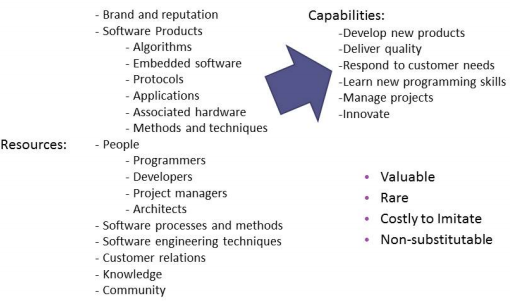
\includegraphics[width=.8\textwidth]{resource_based_theory.png}
  \end{center}
  \caption{Et eksempel på ressourcer og mulig formåen i Resource Based Theory.}
  \label{rbt_fig}
\end{figure}

\paragraph{Ressourcer:}
Herunder følger en fortegnelse over de ressourcer vores virksomhed har til rådlighed:
\begin{itemize}
\item Team:
  \begin{itemize}
  \item Programmør
  \item Sikkerhedsekspert (konsulent)
  \item Hardwaredesigner
  \item Sælger
  \item Systemarkitekt
  \item Usability (konsulentfirma)
  \end{itemize}
\item Produkter
  \begin{itemize}
  \item NFC kort
  \item Fysisk login portal
  \item Software klient -- ansattes pcs kommunikation med NFC kortet
  \item Server sofware -- deling og håndtering af passwords og licenser
  \item Sikkerhedsprotokol mellem fysisk login portal og server
  \item Sikkerhedsprotokol mellem klient og NFC kort
  \item Sikkerhedsprotokol mellem fysisk login portal og NFC kort
  \end{itemize}
\item Pakkeløsning
\item Kundeservice
  \begin{itemize}
  \item Opsætning
  \item Udvidelse
  \item Support
  \end{itemize}
\item Viden om:
  \begin{itemize}
  \item Sikkerhed
  \item Kunders (virksomheder) workflow
  \item Softwarearkitektur
  \end{itemize}
\item Demo setup - som kan bruges til fremføring og test
\end{itemize}
\paragraph{Beskrivelse af team}
Vores team består af os selv, fire mand som står for:
\begin{itemize}
\item Systemarkitektur(hardware og software)
\item Til dels sikkerhed
\item Software
\item Support
\end{itemize}
Udover det består det af en sælger, en hardwaredesigner, en sikkerhedskonsulent og et konsulentfirma til evaluering af usability af produktet.

\paragraph{Formåen:}
Det giver os en mulighed for at levere en samlet løsning, skræddersyet til kunden som samtidig er sikker at bruge.
Det er en løsning hvormed der satses på god usability, og at det ikke forstyrrer de ansatte i deres daglidag, ved fx at ændre deres workflow.
De ansatte skal ikke tænke på sikkerhed men data er alligevel beskyttet af sikre passwords.
